\section{Conclusion}

\begin{figure}[H]
	\hspace{-1cm}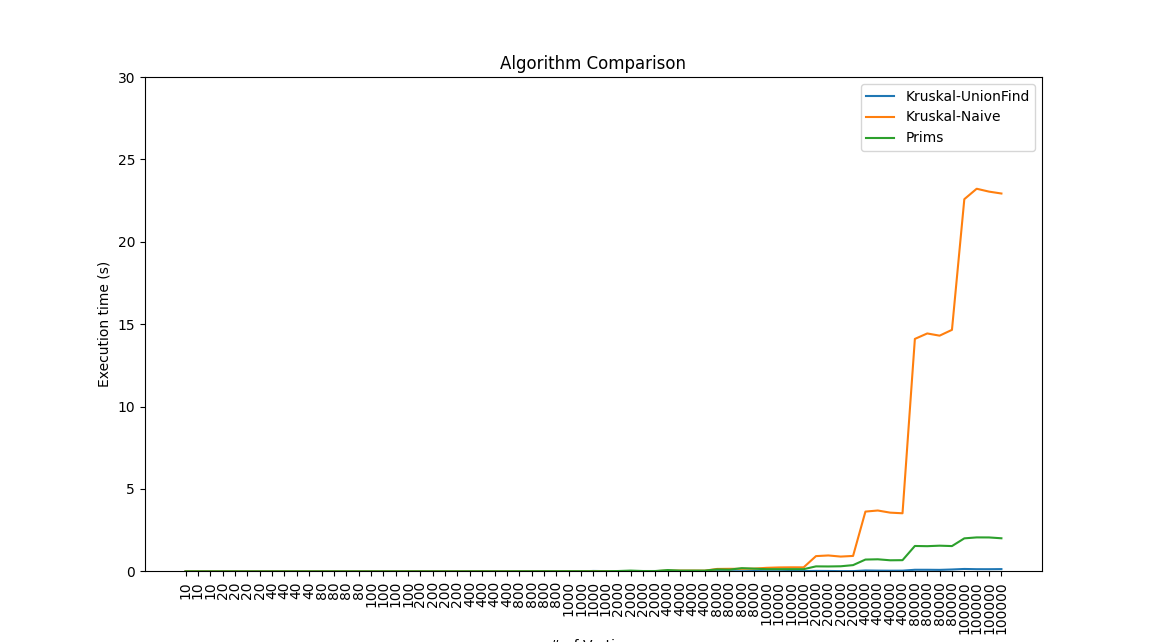
\includegraphics[width=19cm]{Img/AlgorithmComparison_Graph.png}
	\caption{Comparison between the performances of the three algorithms }
	\label{comparison}
\end{figure}

From Fig.~\ref{comparison} we can observe that for graphs with $1000$ vertices or less the performance is more or less the same for the three different algorithms.
As the number of vertices grows, the execution time of the Kruskal's ''naive'' algorithm grows exponentially and it can take nearly a minute to calculate the MST of the larger graphs within the dataset.
The execution time of Prim's and Kruskal's Union Find are very similar.
Prim's only takes a few seconds, and Kruskal's Union Find takes even less than a second, to calculate the MST of the larger graphs within the dataset. 
The results are consistent with the complexity of the algorithms.
Kruskal's ''naive'' is the most complex algorithm, and while the other two have the same algorithmic complexity we still find that the Kruskal's Union Find has an execution time lower than Prim's.


\pagebreak